\documentclass{beamer}
\usetheme{Warsaw}
\usepackage[T1]{fontenc}                                                            % fonte
\usepackage[utf8]{inputenc}                                                         % codificação do arquivo tex, caracteres utf8
\usepackage[brazil]{babel}                                                          % hifenização
\usepackage{graphicx}                                                               % imagens e gráficos graphviz
\usepackage{amsmath}                                                                % equações
\usepackage{mathtools}                                                              % mais símbolos matemáticos
\usepackage{amssymb}                                                                % símbolos, como flechas e outros
\usepackage{mathrsfs}                                                               % símbolos extras com comando \mathscr, ex: símbolos para transformadas F, Z e L
\usepackage{siunitx}                                                                % unidades SI

% Listagem de código fonte
\usepackage{listings}

\makeatletter
\lst@Key{source}{}{\def\lst@source{#1}} % adicionar opção de fonte
\lst@Key{sourcePrefix}{}{\def\lst@sourcePrefix{#1}} % adicionar opção de prefixo da fonte. Ex: 'Fonte: '

\let\orig@lst@MakeCaption=\lst@MakeCaption % redefinir comando de caption para códigos
\def\lst@MakeCaption#1{%
    \orig@lst@MakeCaption#1%
    \ifx b#1%
        \ifx\lst@source\@empty\else
            \noindent
            \vskip\belowcaptionskip
            \expandafter\lst@makesourcebox\expandafter{\lst@sourcePrefix{} \lst@source{}}%
        \fi
    \fi
}

\def\lst@makesourcebox#1{ % caixa para receber a legenda inferior da fonte
    \makebox[\linewidth][c]{
        \fontfamily{\familydefault}\selectfont
        \footnotesize #1
    }%
}
\makeatother

% estilo da listagem de código
\definecolor{background_color}{HTML}{f8f8fd}
\definecolor{comment_color}{HTML}{6AAF19}
\definecolor{keyword_color}{HTML}{F92672}
\definecolor{ndkeyword_color}{HTML}{00FF00}
\definecolor{string_color}{HTML}{F25A00}
\definecolor{identifier_color}{HTML}{000000}
\definecolor{line_number_color}{HTML}{000000}
\lstdefinestyle{mystyle}{
    backgroundcolor=\color{background_color},   
    commentstyle=\color{comment_color},
    keywordstyle=\color{keyword_color},
    ndkeywordstyle=\color{ndkeyword_color},
    numberstyle=\tiny\color{line_number_color},
    stringstyle=\color{string_color},
    identifierstyle=\color{identifier_color},
    basicstyle=\ttfamily\footnotesize,
    breakatwhitespace=false,         
    breaklines=true,                 
    keepspaces=true,                 
    numbers=left,                    
    numbersep=5pt,                  
    showspaces=false,                
    showstringspaces=false,
    showtabs=false,                  
    tabsize=2,
    captionpos=t,
    aboveskip=15pt,
    belowskip=15pt,
    belowcaptionskip=1ex,
    xleftmargin=1em,
    numbersep=0.5em,
    numberbychapter=false
}
\renewcommand\lstlistingname{Código}
\renewcommand\lstlistlistingname{Lista de códigos}
\lstset{style=mystyle}   

% generated by the Super Figure vscode extension. May we stand on the shoulder's of giants
\usepackage{import}
\newcommand{\incsvg}[2]{%
	\def\svgwidth{\columnwidth}
	\graphicspath{{#1}}
	\input{#2.pdf_tex}
}

%% ---------------------------------------------------- main body --------------------------------------------

\title{Desenvolvimento de um método e sistema para compilação e simulação de redes de petri para utilização em controladores lógicos industriais}
\author{João Peterson Scheffer}

\begin{document}
\maketitle

\section{Introdução}

\begin{frame}
\frametitle{Introdução}

	\begin{itemize}
		\item Automação industrial
		\item PLC's 
		\begin{itemize}
			\item \textit{Ladder}
			\item Lista de instrução
			\item SCL
			\item SFC
		\end{itemize}
		\item Redes de Petri
	\end{itemize}
\end{frame}

\begin{frame}
\frametitle{Redes de Petri}

\begin{figure}[ht]
	\centering
	\caption{Exemplo de rede de petri}
	\scriptsize
	%\incsvg{path/}{path/file}
	\incsvg{images}{images/pnetcomp}\\
	\label{fig:pnetcomp}
	\footnotesize{Fonte: Do autor.}
\end{figure}
\end{frame}

\begin{frame}
\frametitle{Justificativa}

	\begin{itemize}
		\item Ferramentas
		\begin{itemize}
			\item Edição 
			\item Simulação / Execução
			\item Compiladores
		\end{itemize}
	\end{itemize}
\end{frame}

\begin{frame}
\frametitle{Objetivos}

	\begin{itemize}
		\item Desenvolvimento de uma biblioteca implementada em linguagem C que deve implementar os seguintes pontos: 
		\begin{itemize}
			\item Estrutura de dados.
			\item Serialização de dados para armazenamento.
			\item Capacidade de checagem e validação.
			\item Capacidade de execução normal e temporizada de forma assíncrona.
		\end{itemize}
		
		\item Desenvolvimento de algoritmos de compilação de redes de petri para os seguintes alvos:
		\begin{itemize}
			\item Lista de instrução, em formato de texto para a referência PLC WEG TPW04.
		\end{itemize}
	\end{itemize}

\end{frame}

\section{Fundamentação}

\begin{frame}
\frametitle{Delimitação da rede}
\begin{columns}
	\column{.5\textwidth}
	Tipos:
	\begin{itemize}
		\item Redes de petri coloridas
		\item Redes de petri temporizadas
		\item Redes de petri estocásticas
		\item Redes de petri priorizadas
		\item Redes de petri de alto nível
	\end{itemize}
	
	\column{.5\textwidth}
	Funcionalidade:
	\begin{itemize}
		\item Entradas 
		\item Saídas 
		\item Arcos de peso 
		\item Arcos negados / de inibição 
		\item Arcos de reset
		\item Transições temporizadas 
	\end{itemize}
\end{columns}
\end{frame}

\begin{frame}
\frametitle{Arcos de peso}
	\begin{figure}[ht]
		\centering
		\caption{Exemplo de arco de peso}
		\incsvg{images}{images/samplepetri}\\
		\label{fig:sampepetri}
		\footnotesize{Fonte: Do autor.}
	\end{figure}
\end{frame}

\begin{frame}
\frametitle{Transições temporizados}
\begin{figure}[ht]
	\centering
	\caption{Exemplo de transição temporizada}
	\incsvg{images}{images/petritime}\\
		\label{fig:sampepetri}
		\footnotesize{Fonte: Do autor.}
	\end{figure}
\end{frame}

\begin{frame}
\frametitle{Arcos negados / de inibição}
\begin{figure}[ht]
	\centering
		\caption{Exemplo de arco negado}
		\incsvg{images}{images/negado}\\
		\label{fig:sampepetri}
		\footnotesize{Fonte: Do autor.}
	\end{figure}
\end{frame}

\begin{frame}
\frametitle{Arcos de reset}
\begin{figure}[ht]
	\centering
	\caption{Exemplo de arco de reset}
	\incsvg{images}{images/reset}\\
	\label{fig:sampepetri}
	\footnotesize{Fonte: Do autor.}
\end{figure}
\end{frame}

\begin{frame}
\frametitle{Implementação}
\begin{columns}
	\column{.5\textwidth}
	Formas:
	\begin{itemize}
		\item Forma relacional
		\item Forma matricial
	\end{itemize}
	\column{.5\textwidth}
	Matrizes:
	\begin{itemize}
		\item Arcos de peso
		\item Arcos negados e reset
		\item Temporização das transições
		\item Marcação inicial
		\item Eventos de entrada
		\item Condições de saída
	\end{itemize}
\end{columns}
\end{frame}

\begin{frame}
\frametitle{Matrizes}

	Rede de petri de 2 transições por 3 lugares:

	$$ A_p =
	\begin{bmatrix}
		-1 & 0\\
		0 & -1\\
		0 & 0
	\end{bmatrix}
	$$

	$$ A_n =
	\begin{bmatrix}
		0 & 0\\
		1 & 0\\
		0 & 2
	\end{bmatrix}
	$$

	$$
	P_i = 
	\begin{bmatrix}
		1 & 0 & 0
	\end{bmatrix}
	$$

	
	% \resizebox{!}{3.5cm}{
	% 	\lstinputlisting[
	% 		language=C,
	% 		caption={Inicialização de uma rede de petri de forma matricial},
	% 		sourcePrefix={Fonte: },
	% 		source={Do autor.},
	% 		label=code:pnetnew
	% 	]{../code/pnetnew.c}
	% }
\end{frame}

\begin{frame}
\frametitle{Limitações e comportamento}

	\begin{itemize}
		\item Entrada
		\item Disparos simultâneos
		\item Temporização
	\end{itemize}
\end{frame}

\begin{frame}
\frametitle{Lista de instrução}
	\footnotesize
	\begin{figure}[ht]
		\centering
		\caption{Equivalência entre LI e \textit{Ladder}}
		\incsvg{images}{images/illadder}\\
		\label{fig:illadder}
		\footnotesize{Fonte: Do autor.}
	\end{figure}
\end{frame}

\section{Desenvolvimento}

\begin{frame}
\frametitle{Metodologia}
\begin{itemize}
	\item Desenvolvimento da biblioteca C ``pnet''
	\item Desenvolvimento do compilador para IL
\end{itemize}
\end{frame}

\begin{frame}
\frametitle{Sensibilização}
Condições:
\begin{itemize}
	\item Evento de entrada
	\item Arcos de peso negativo
	\item Arcos negados
\end{itemize}
Ação:
\begin{itemize}
	\item Sensibilização única
	\item Fila de temporização
\end{itemize}
\end{frame}

\begin{frame}
\frametitle{Disparo}

\begin{itemize}
	\item Disparo único
	\item Arcos de peso negativo
	\item Arcos de peso positivo
	\item Arcos de reset
\end{itemize}
\end{frame}

\begin{frame}
\frametitle{Arquivo ``.pnet''}
\begin{figure}[h!]
	\centering
	\caption{Visão do arquivo pnet em um analisador hexadecimal}
	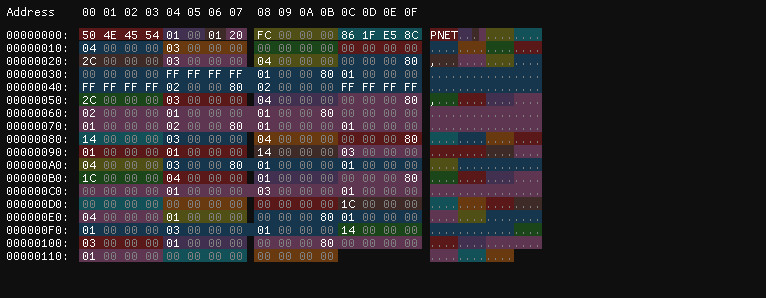
\includegraphics[height=4cm]{images/hexfile.png}
	\label{fig:hexfile}
	\footnotesize{Fonte: Do autor.}
\end{figure}
\end{frame}

\begin{frame}
\frametitle{Compilação para LI}
\begin{figure}[ht]
	\centering
	\caption{Rede de petri exemplo para compilação}
	\scriptsize
	%\incsvg{path/}{path/file}
	\incsvg{images}{images/pnetcomp}\\
	\label{fig:pnetcomp}
	\footnotesize{Fonte: Do autor.}
\end{figure}
\end{frame}

\begin{frame}
\frametitle{Memórias}
\begin{itemize}
	\item Transições \rightarrow \lstinline{M}
	\item Lugares \rightarrow \lstinline{D}
	\item Entradas \rightarrow \lstinline{X}
	\item Saídas \rightarrow \lstinline{Y}
\end{itemize}
\end{frame}

\begin{frame}
\frametitle{Marcação inicial}

\lstinputlisting[
	language=C,
	caption={Exemplo de lista de instrução - Marcação inicial},
	sourcePrefix={Fonte: },
	source={Do autor.},
	firstline=1,
	lastline=2,
	label=code:ilmem
]{code/il.txt}
\end{frame}

\begin{frame}
\frametitle{Sensibilização}

\lstinputlisting[
	language=C,
	caption={Exemplo de lista de instrução - Sensibilização},
	sourcePrefix={Fonte: },
	source={Do autor.},
	firstline=18,
	lastline=20,
	label=code:ilsense
]{code/il.txt}
\end{frame}

\begin{frame}
\frametitle{Sensibilização com temporizador}

\lstinputlisting[
	language=C,
	caption={Exemplo de lista de instrução - Sensibilização com temporizador},
	sourcePrefix={Fonte: },
	source={Do autor.},
	firstline=8,
	lastline=15,
	label=code:iltimer
]{code/il.txt}
\end{frame}


\begin{frame}
\frametitle{Disparo das transições}

\lstinputlisting[
	language=C,
	caption={Exemplo de lista de instrução - Disparo das transições},
	sourcePrefix={Fonte: },
	source={Do autor.},
	firstline=67,
	lastline=75,
	label=code:ilfire
]{code/il.txt}
\end{frame}

\begin{frame}
\frametitle{Saídas}

\lstinputlisting[
	language=C,
	caption={Exemplo de lista de instrução - Saídas},
	sourcePrefix={Fonte: },
	source={Do autor.},
	firstline=76,
	lastline=78,
	label=code:ilout
]{code/il.txt}
\end{frame}

\section{Conclusão}

\begin{frame}
\frametitle{Conclusão}
\begin{itemize}
	\item Commits realizados: 42
 	\item Arquivos: 21
 	\item Linhas comentadas de código: 947
 	\item Linhas de código escrito: 3368
	\item Período de trabalho: Maio 2022 - Junho 2023
\end{itemize}
\end{frame}

\begin{frame}
\frametitle{Trabalhos futuros}
\begin{itemize}
	\item Editor gráfico
\end{itemize}
\end{frame}


% \begin{figure}[ht]
% 	\centering
% 	\caption{}
% 	\incsvg{images}{images/comedor}\\
% 	\label{fig:teste}
% 	\footnotesize{Fonte: Do autor.}
% \end{figure}

\end{document}